\documentclass{scrartcl}
\setkomafont{disposition}{\normalfont\bfseries}
\usepackage[utf8]{inputenc}
\usepackage{natbib}
\usepackage{graphicx}
\usepackage[francais]{babel}
\usepackage[T1]{fontenc}
\usepackage{xcolor}
\usepackage{hyperref}
\usepackage{amsmath}
\usepackage{listings}
\usepackage{calc}
\usepackage{xparse}
\usepackage{framed}
\usepackage{amssymb}
\usepackage{amsfonts}
\usepackage{tabularx}
\usepackage{makecell}
\usepackage{float}
\usepackage[toc,page]{appendix}
\usepackage[nottoc]{tocbibind}
\renewcommand\appendixtocname{Annexes}
\renewcommand\appendixpagename{Annexes}

\lstset{ 
  basicstyle=\footnotesize,
  commentstyle=\color{green},
  frame=single,
  keywordstyle=\color{blue},
  language=Java,
  rulecolor=\color{black},
  stringstyle=\color{red},
  tabsize=2,
  title=\lstname
}

\newcommand{\project}{$\mathbf{\Pi}$}
\newcommand{\classUniverse}{$\mathbf{U}$}
\newcommand{\category}{$\mathbf{C}$}
\newcommand{\class}{$c$}

\newcommand{\categoryUniverse}{$\mathbf{P}$}
\newcommand{\dependantClasses}{$\mathbf{DaC}$}
\newcommand{\dependedClasses}{$\mathbf{DeC}$}
\newcommand{\numberOfMethod}{$\mathbf{NoM}$}
\newcommand{\numberOfabstractMethod}{$\mathbf{NoAM}$}

% Macro structuration des besoins. Trois arguments (dans l'ordre) :
% - Titre;
% - Priorité (Faible, Moyenne ou Forte);
% - Description;
\newcommand{\requirement}[3] {
    \vbox{
        \begin{framed}
            {\centering \textbf{\underline{#1}}\\[0.25 cm]\par}
            \begin{itemize}
                \item \textbf{Priorité} : #2
                \item \textbf{Description} : #3
            \end{itemize}
        \end{framed}
    }
}

\newcommand{\TODO}[1] {
    \noindent \paragraph{\textcolor{red}{#1}}
}

\title{Mémoire}
\author{Delrée Sylvain, Giachino Nicolas, Martinez Eudes, Ousseny Irfaane}
\date{Jeudi 4 Avril 2019}
\makeatletter
\let\thetitle\@title
\let\theauthor\@author
\let\thedate\@date
\makeatother

\begin{document}

\begin{titlepage}
	\centering
    \vspace*{0.5 cm}
    
\includegraphics[scale = 0.5]{img/logo.jpg}\\[1.0 cm]
    \textsc{\LARGE PdP - Métriques de Maintenabilité}\\[1.0 cm]
	\rule{\linewidth}{0.2 mm} \\[0.4 cm]
	{\huge \bfseries \thetitle}\\
	\rule{\linewidth}{0.2 mm} \\[0.5 cm]
	{\small \thedate}\\[0.5 cm]
	{\small Dépôt Savane :\\ \url{https://services.emi.u-bordeaux.fr/projet/savane/projects/pdp2019mm/}}\\[1.5 cm]
	\begin{minipage}{0.4\textwidth}
		\begin{flushleft} \large
			\emph{Soumis pour :}\\
			(Client) Narbel Philippe\\
            (Chargé de TD) Hofer Ludovic\\
		\end{flushleft}
	\end{minipage}~
	\begin{minipage}{0.4\textwidth}
        \begin{flushright} \large
			\emph{Soumis par :} \\
			Delrée Sylvain\\
            Giachino Nicolas\\
            Martinez Eudes\\
            Ousseny Irfaane\\
		\end{flushright}
	\end{minipage}\\[2 cm]
\end{titlepage}
\tableofcontents
\pagebreak










                    % ------------------------------------- %
                    % -------------> CONTENT <------------- %
                    % ------------------------------------- %

\section{Introduction}
    
    \TODO{Phrase d'accroche}

    \paragraph{}Dans ce contexte, étudier en profondeur les éléments qui semblent rendre un design flexible, robuste et maintenable ainsi que fournir des outils qui permettent l'extraction et l'analyse de ces éléments constitue une priorité. En effet, être capable de déterminer le degré de maintenabilité d'un projet permettrait aux développeurs d'effectuer un suivi de la qualité de leur application. Ceci rendrait le développement et la maintenance plus aisés.

    \paragraph{}Dans le cadre de l'unité d'enseignement \og Projet de Programmation\fg, la métrique définie par Martin\cite{Martin:1994} va être au centre de notre projet. Cette dernière permet, au travers d'une analyse des dépendances, une étude sur la maintenabilité d'un projet de développement logiciel.

    \paragraph{}Dans le cas de notre projet, l'application reçoit en entrée un programme de paradigme Orienté Objet à analyser. L'application que nous devrons mettre en oeuvre devra réaliser une analyse au moyen de métriques logicielles afin d'obtenir des informations sur la maintenabilité en sortie.

\begin{figure}[ht]
    \centering
    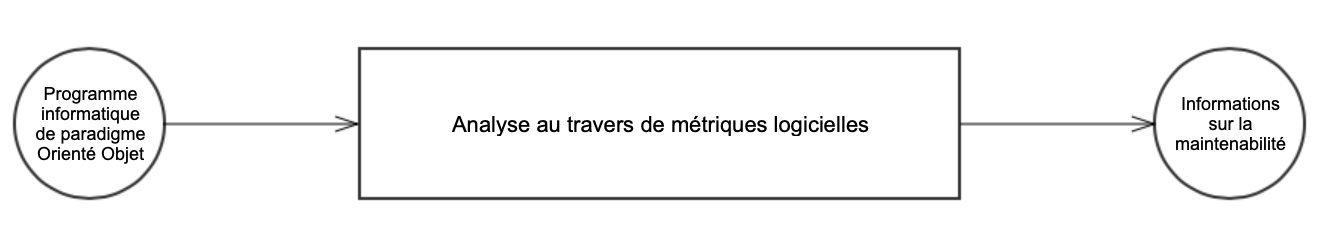
\includegraphics[scale=0.65]{img/intro.png}
    \caption{Vision simplifiée du fonctionnement de l'application} 
    \label{fig:intro}
\end{figure}
    




                    % ------------------------------- %
                    % ----------> DOMAINE <---------- %
                    % ------------------------------- %

\newpage
\section{Description du domaine}

    \begin{abstract}
        Cette section a pour vocation de décrire la métrique utilisée ainsi que tout le vocabulaire nécessaire à sa compréhension.
    \end{abstract}

\subsection{Préambule}

    \paragraph{}Le domaine dans lequel s'inscrit l'application est celui de l'architecture logicielle. En effet, il s'agit ici de déterminer un indicateur du degré de qualité qu'un logiciel possède au regard de la manière dont sont structurés ses composants. Bien que de nombreuses métriques aient été élaborées dans ce but, le programme s'appuiera sur celle définie par Robert Martin\cite{Martin:1994}. Cette étude s'intéressera à son application au paradigme orienté objet. 
    
\subsection{Concepts}
\label{mm:concepts}

\subsubsection{Dépendances et granularités}
    \paragraph{Granularité}La granularité est une échelle de groupement hiérarchique des éléments constitutifs d'un programme. Chaque niveau de granularité est une partition de l'ensemble de ces éléments. Des exemples de niveaux de granularité dans un programme orienté objet sont :
    \begin{itemize}
        \item Les attributs et méthodes.
        \item Les classes et objets.
        \item Les packages, les namespaces.
        \item Les super-packages.
    \end{itemize}
    Les éléments d'un niveau de granularité sont appelés \textbf{granules}. Chaque granule d'un niveau contient un ensemble de granules du niveau du dessous.
    
    \paragraph{Dépendance}Soient A et B des granules, le plus souvent du même niveau. A \emph{dépend} de B dans le cas où A utilise B dans sa définition. Cette relation de dépendance peut s'exprimer sous différentes formes :
    \begin{itemize}
        \item \textbf{Dépendance par héritage} : A est de type B.
        \item \textbf{Dépendance par association} : A possède un attribut de type B.
        \item \textbf{Dépendance par usage} : A communique avec B. 
    \end{itemize}

    \paragraph{Couplage}Le degré de couplage est une mesure de l'\emph{interdépendance} entre les différents composants d'un programme. On parle de couplage fort pour signifier que l'interdépendance est élevée.

    \paragraph{Cohésion}La cohésion représente le degré de liaison, de collaboration et d'interdépendance entre les éléments appartenant à un même granule. Une forte cohésion implique que le composant se concentre sur un seul et unique but, une seule et même responsabilité : réaliser des traitements relatifs uniquement à l’intention du composant.
    
    \paragraph{Principe de simplification min-max}Pour deux niveaux de granularité consécutifs, il faut favoriser une cohésion forte et un couplage faible.

\subsubsection{Propriétés d'un design}

    \paragraph{}Afin de comprendre la métrique détaillée dans ce document, il est nécessaire de définir plusieurs propriétés qu'une architecture logicielle peut posséder (ceux-ci sont repris de l'article fondateur de cette métrique, définie par Robert Martin\cite{Martin:1994}) :

    \paragraph{Rigidité}Un design rigide est un design qui ne peut être facilement changé. C'est souvent le cas si les composants d'un système sont trop interdépendants. Dans ce cas, un changement dans un composant peut forcer beaucoup d'autres composants à changer également et son impact peut être difficile, si ce n'est impossible, à évaluer.

    \paragraph{Fragilité}Un design fragile est un design qui a tendance à cesser de fonctionner à plusieurs endroits si un seul changement est effectué. Dans la plupart des cas, les problèmes engendrés par cette modification surviennent à des endroits sans relation conceptuelle avec la partie ayant subi la modification. De plus, la correction de ces erreurs amène souvent à davantage de nouveaux problèmes.

    \paragraph{Robustesse}Un design robuste est l'exact opposé d'un design fragile. En effet, est considéré comme robuste un design au sein duquel un unique changement ne cause pas tout une cascade de problèmes.

    \paragraph{Maintenabilité}Un design maintenable est un design qui peut facilement évoluer. Il faut comprendre par là qu'il doit être facile d'ajouter de nouvelles fonctionnalités ou de modifier le comportement de celles déjà existantes. Un design rigide ou fragile sera peu maintenable.

    \paragraph{Réutilisabilité}Un design réutilisable est un design qui permet la réutilisation de certains de ses composants sans nécessiter d'embarquer ceux dont on ne veut pas. Si ses composants dépendent fortement les uns des autres, le design est dit difficile à réutiliser car il est compliqué d'isoler les composants désirés.
    
\subsubsection{Propriétés d'un composant}
\label{componentProperties}

    \paragraph{}Il s'agit ici de définir plusieurs propriétés que peuvent avoir les composants d'un logiciel. Ces propriétés interviennent dans le calcul de la métrique détaillée plus bas.
    
    \paragraph{Responsabilité}Un composant responsable est un composant dont dépendent d'autres composants. Un tel composant a intérêt à ne pas être souvent modifié car chaque changement peut se diffuser aux composants dépendant de lui.
    
    \paragraph{Indépendance}Un composant est dit indépendant s'il ne dépend d'aucun autre. Cette notion peut être nuancée : on peut admettre qu'un composant est très indépendant s'il dépend de peu d'autres et peu indépendant s'il dépend de beaucoup d'autres. Un composant très indépendant sera peut amené à changer à cause d'autres composants, de par son faible nombre de dépendances.
    
    \begin{figure}[ht]
        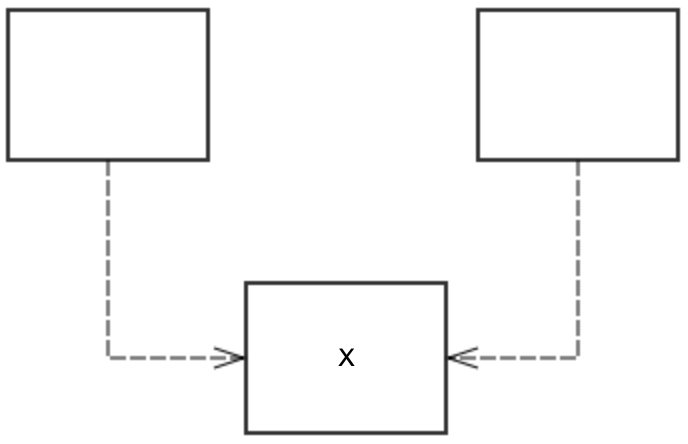
\includegraphics[width=\textwidth/2]{img/StableGranule.png}
        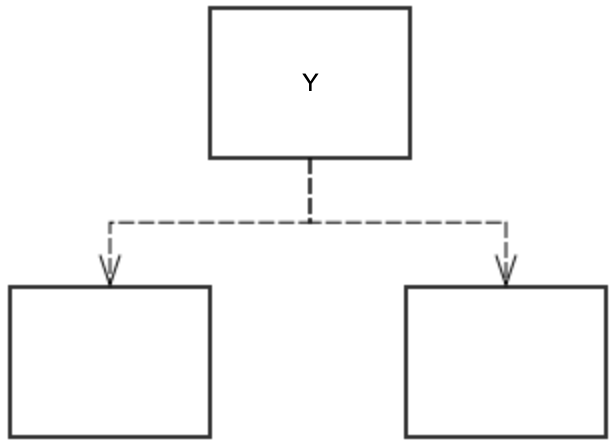
\includegraphics[width=\textwidth/2]{img/InstableGranule.png}
        \caption{Un granule stable X et un granule instable Y}
    \end{figure}
    
    
    \paragraph{Stabilité}La stabilité est une propriété combinant les deux précédentes. En effet, joue en faveur de la stabilité d'un composant :
    \begin{itemize}
    	\item Le nombre de composants dépendant de lui (\emph{responsabilité}).
    	\item L'absence de composants dont il dépend (\emph{indépendance}).
    \end{itemize}
    La combinaison d'une forte responsabilité et d'une importante indépendance est synonyme de forte stabilité et vice versa. La stabilité vise à fournir une indication de la tendance qu'un composant aura à changer dans le temps. Plus le composant est stable, plus cette tendance est faible. En effet, un composant responsable aura peu tendance à changer à cause de la propagation des changements que cela peut engendrer. De même, un composant indépendant aura moins tendance à changer que s'il avait beaucoup de dépendances car une modification extérieure a peu de chances de se répercuter sur lui.
    
    \paragraph{Stable Dependency Principle (SDP)}Selon le SDP, énoncé par Martin\cite{Martin:2003}, une bonne dépendance (\emph{Good dependency}) est une dépendance dont la cible est très stable. Si A dépend de B et que B est très stable, alors cette dépendance est très bonne. Par opposition, une mauvaise dépendance (\emph{Bad dependency}) est une dépendance dont la cible est instable. Ce sont, assez naturellement, ces dépendances qu'il faut éviter.
   
    \paragraph{Niveau d'abstraction}L'abstraction, ou le niveau d'abstraction, désigne la proportion d'un composant qui est abstraite (c.à.d. une partie ne comportant que des signatures et pas d'implémentation, dans le but d'être héritée et définie ailleurs). Plus un composant contient de parties abstraites par rapport à sa taille totale, plus il est lui-même abstrait.

\subsection{Métrique de Martin}
\subsubsection{Présentation et définitions}

    \paragraph{}La métrique de Martin a été définie pour la première fois en 1994 par Robert Martin\cite{Martin:1994}. L'auteur l'a par la suite citée au sein d'autres ouvrages\cite{Martin:2003}, et une large bibliographie scientifique mentionne, critique et complète celle-ci\cite{HyryLepp:2009}\cite{BUmetric:2016}\cite{KaurShar:2015}\cite{Spinellis:2006}\cite{Pressman:2000}. La métrique s'articule autour de 2 notions centrales : la stabilité et le niveau d'abstraction (cf. \ref{componentProperties}).


    \paragraph{Composantes}Martin présente une métrique principale : la distance entre un \textit{granule} représenté par un point de coordonnées (Instabilité, Abstraction) et la \emph{Main Sequence}, une droite représentant le positionnement idéal des granules. Plus cette distance est grande, moins le granule correspond au modèle recherché. Afin de calculer cette distance, il est nécessaire de calculer plusieurs autres métriques, qui s'appliquent toutes à un granule :
    \begin{itemize}
        \item \textbf{Afferent Coupling} (couplage afférent), noté \textbf{Ca} : Il s'agit du nombre de granules externes qui dépendent du granule.
        \item \textbf{Efferent Coupling} (couplage efférent), noté \textbf{Ce} : Il s'agit du nombre de granules externes dont dépend le granule.
        \item \textbf{Instability} (instabilité), notée \textbf{I} : Il s'agit d'une quantification de la stabilité du granule (cf. \ref{mm:concepts}). Cette métrique fait intervenir les deux précédentes.
        \item \textbf{Abstractness} (niveau d'abstraction), noté \textbf{A} : Il s'agit d'une quantification du niveau d'abstraction du granule.
        \item \textbf{Distance} (Distance par rapport à la Séquence Principale), notée \textbf{D} (ou \textbf{Dn} pour la version normalisée) : Il s'agit d'une mesure de la distance perpendiculaire du granule à la Séquence Principale. Cette distance donne une idée de la qualité du granule : le but est de minimiser cette valeur.
    \end{itemize}

\begin{figure}[ht!]
    \centering
    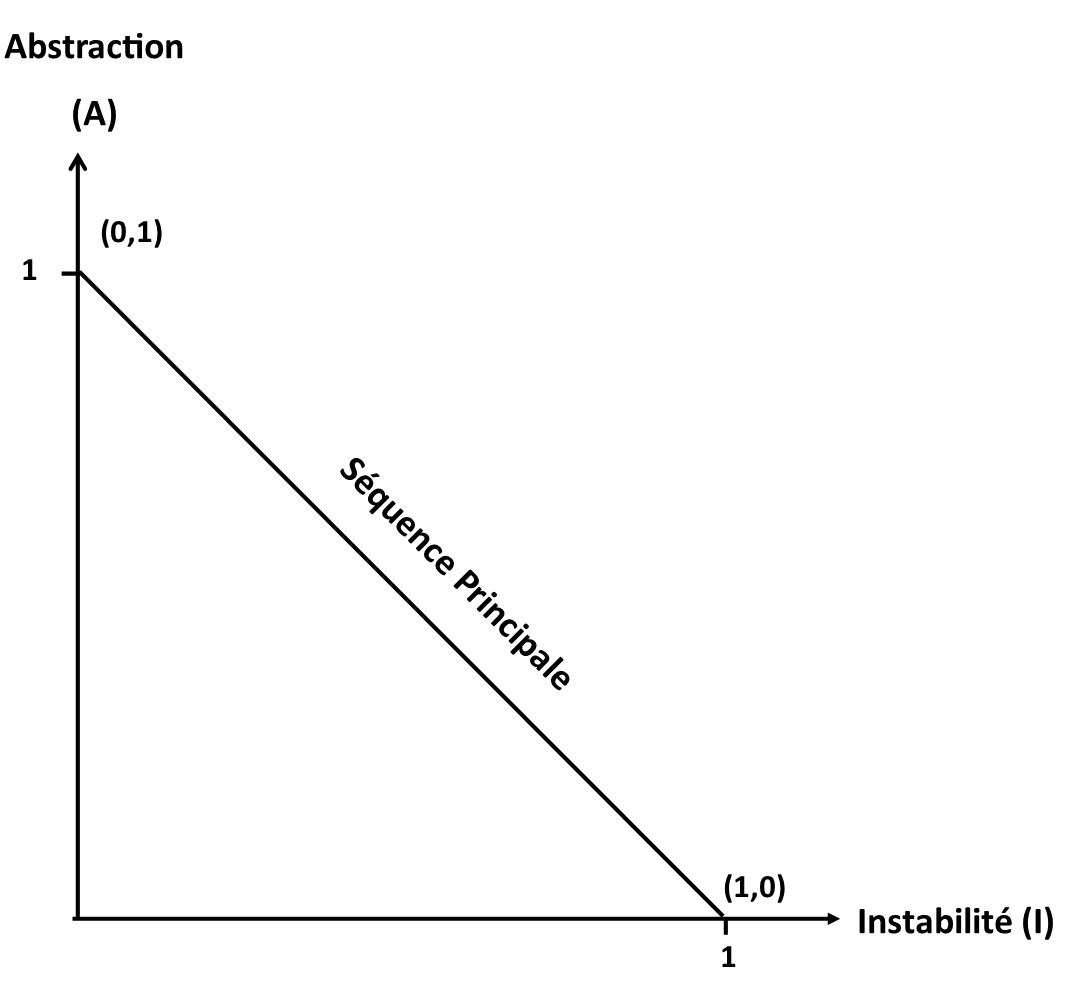
\includegraphics[scale=0.2]{img/MainSequence.png}
    \caption{Séquence principale}
\end{figure}

    \paragraph{}Il est également nécessaire de définir ce qu'est la \textbf{Séquence Principale} (\emph{Main Sequence}). Elle intervient dans le contexte d'une représentation en deux dimensions des métriques. Dans ce plan, un granule est représenté par un point dont les coordonnées sont les suivantes : \textbf{(Instabilité, Niveau d'Abstraction)}. Les positions idéales se situent en coordonnées (0,1) : il s'agit d'un granule instable mais entièrement concret ; ainsi qu'en (1,0) : il s'agit d'un granule très stable et entièrement abstrait. Des compromis sont également possibles : il s'agit de la Séquence Principale, une droite passant par (0,1) et (1,0). Les granules proches de cette droite sont considérées comme bien équilibrées.
    


\subsubsection{Formalisme}
\TODO{FORMALISME}
    % \TODO{Dans la suite, il sera souvent fait référence à l'\textbf{instabilité}, qui est simplement la mesure contraire à la stabilité. En effet, elles sont toutes deux comprises entre 0 et 1 et la relation suivante permet de passer de l'une à l'autre : \emph{instabilité = 1 - stabilité}.}
% \TODO{Voir avec Narbel si on conserve}
% \label{martin:formalism}

%     \paragraph{Variables}Soit \project{} un projet de développement. Un projet \project{} est composé par un ensemble de $n$ ($n > 0$) classes et de $m$ ($m \geq 0$) packages. On note \classUniverse{}, l'univers des classes. \classUniverse{} = $\{\class{}_1, \class{}_2, \dots, \class{}_n\}$ où $c_1, c_2, ... c_n$ représentent les $n$ classes de \project.

%     Une catégorie \category{} est un sous-ensemble non-vide de U : \category{} = $ \{\class{}_i, \dots, \class{}_j\} \subseteq$ \classUniverse{}, avec $0 > i, j \geq n$.

%     On définit \categoryUniverse{} comme l'ensemble des \category{}. On appelle catégorie élémentaire une catégorie de cardinal 1 (c.à.d. une catégorie composée d'une unique classe).

%     \paragraph{Fonctions}On note les fonctions suivantes :
%     \begin{itemize}
%         \item \dependantClasses{}(\category{}) = Le nombre de classes dépendant d'une catégorie \category{}.
%         \item \dependedClasses{}(\category{}, \categoryUniverse{}) = Le nombre de classes dont dépend une catégorie \category{} dans son univers \categoryUniverse{}.
%         \item \numberOfMethod{}(\category{}) = Le nombre de méthodes présentes au sein d'une catégorie \category{}.
%         \item \numberOfabstractMethod{}(\category{}) = Le nombre de méthodes abstraites présentes au sein d'une catégorie \category{}.
%     \end{itemize}

%     \paragraph{Calculs}Les différentes métriques définies plus haut sont calculables par application des formules suivantes : 
%     \begin{itemize}
%         \item Ca(\category{}) = \dependantClasses{}(\category{}) $\in \mathbb{N}$
        
%         \item Ce(\category{}, \categoryUniverse{}) = \dependedClasses{}(\category{}, \categoryUniverse{}) $\in \mathbb{N}$
        
%         \item A(\category{}) = 
%         \numberOfabstractMethod{}(\category{}) /
%         {\numberOfMethod{}(\category{})} $\in \lvert 0, 1\rvert$

%         \item I(\category{}) = Ce(\category{}) / (Ca(\category{}) + Ce(\category{})) $\in \lvert 0, 1\rvert$
        
%         \item \textbf{D(\category{}) = | (A + I - 1) / $\sqrt{2}$ | $\in \lvert 0, 0.707\rvert$}
%     \end{itemize}
    
% La distance peut se normaliser dans un intervalle de 0 à 1 en utilisant une formule simplifiée :
% \begin{itemize}
%     \item Dn(\category{}) = | (A(\category{}) + I(\category{}) - 1) | $\in \lvert 0, 1\rvert$.
% \end{itemize}


\subsection{Intérêts}

    \paragraph{Comprendre la métrique}Un intérêt sous-jacent à l'objectif principal de l'application est que son développement est un moyen efficace de comprendre et de mener une réflexion sur la métrique. Ceci permettrait de l'évaluer dans son ensemble afin d'en apporter des améliorations.

    \TODO{Critique et Explication séquence principale (cf. Validation Martin's Metrics article (Page 89 - 90))}
    
    \paragraph{Critique et pistes d'amélioration}Le problème majeur que l'on peut reprocher à toutes les métriques est que le résultat du calcul des métriques ne constituent pas des références absolues, ce sont des indicateurs qui peuvent servir à détecter les zones de code auxquelles prêter une attention particulière.
    

    \paragraph{}Les métriques décrites par Chidamber et Kemerer\cite{ChidamberKemerer:1994} définissent un  indicateur plus simplifié que les métriques de Martin. En effet, ils définissent six métriques telles que la profondeur de l'arbre d'héritage (DIT), le nombre de fils d'une classe (NOC), le manque de cohésion des méthodes d'une classe (LCOM) et bien d'autres qui sont utiles dans l'étude du couplage et la cohésion au niveau de différentes classes. Certains éléments de ces métriques peuvent servir à améliorer la métrique de Martin.
    
    \begin{quote}
        These metrics should assist software designers in their understanding of the complexity of their design and help direct them to simplifying their work. What the designers should strive for is strong cohesion and loose coupling.
        \begin{flushright}--- C. Kemerer \& S. Chidamber \cite{ChidamberKemerer:1994} (p.229)\end{flushright}
    \end{quote}
    
    \paragraph{}Martin présente sa métrique comme ne s'appliquant qu'aux catégories contenant plusieurs classes. Cependant, en utilisant le formalisme exprimé en section \ref{martin:formalism} et l'exemple décrit en annexe, la métrique de Martin peut s'appliquer à l'échelle des classes (granules élémentaires).
    
    \paragraph{}Telle qu'elle est énoncée, la métrique de Martin considère les dépendances comme toutes égales. Or, une dépendance envers un granule stable ne devrait pas avoir le même poids qu'une dépendance envers un granule instable. Afin de raffiner le calcul des métriques, une analyse de la globalité de l'arbre des dépendances permettrait d'éliminer les dépendances stables du calcul d'instabilité (ou du moins de minimiser leur poids), en considérant qu'une dépendance stable ne rend pas le composant dépendant instable. Il s'agit d'une exploitation du SDP.


\subsection{Application au langage Java}

    \paragraph{}L'application aura pour but d'appliquer la métrique à des programmes écrits en langage Java. Dans ce cadre, une clarification de la manière dont certains concepts sont utilisables en Java est nécessaire.

\subsubsection{Adaptation des notions}

    \paragraph{Catégories de classes}La notion la plus proche de catégorie de classes dans le langage Java est celle de package. Cependant, il existe un glissement sémantique : bien que ce soit souvent le cas en pratique, un package Java n'est pas obligatoirement composé d'un ensemble de classes \emph{collaborant} pour offrir un ensemble de services. Cette notion peut aussi s'appliquer aux modules.

\subsubsection{Analyse de l'existant}
    \paragraph{}Il existe différents projets qui abordent la question de la maintenabilité de logiciels au travers de l'étude de métriques (on notera que beaucoup d'entre eux exposent les métriques de Chidamber et Kemerer\cite{ChidamberKemerer:1994}). Pour le langage Java, on peut citer JHawk\footnote{\url{http://www.virtualmachinery.com/jhawkprod.htm}} en guise d'exemple. Certains de ces outils s'intègrent à des IDE comme Eclipse ou IntelliJ, ce qui facilite grandement leur mise en place et leur installation.
    
    \paragraph{JDepend}JDepend est un logiciel open source dont le code source est disponible sur la plateforme Github\footnote{\url{https://github.com/clarkware/jdepend}}. Il met en oeuvre la métrique de Martin (et nourrit donc des ambitions similaires à celles de notre application).

    \paragraph{}JDepend procède à une analyse statique des différents fichiers constituant un projet Java. Plus exactement, il analyse les fichiers compilés (\texttt{.class}) composés de bytecode (il peut également analyser les archives jar).
    
    \paragraph{}A la suite d'une étude du fonctionnement de JDepend, il ressort que celui-ci n'extrait que les informations de dépendance entre les packages. Il extrait les dépendances et calcule ensuite les valeurs de métriques à cette échelle. Il ne peut donc fournir aucune information sur les dépendances entre classes. 
    
    \paragraph{}L'approche du projet décrit dans ce document est différente. En effet, là où JDepend se limite aux packages, notre application adopte une approche \textit{bottom-up} : l'analyse s'effectue au niveau de granularité le plus bas (la classe). A partir des résultats de celle-ci, on peut alors calculer les dépendances et métriques des échelles supérieures sans analyse supplémentaire.
    
    \paragraph{Remarque}Certains travaux se basent sur l'outil JDepend pour analyser des programmes, comme par exemple \textit{Gephi}\footnote{\url{https://dzone.com/articles/visualizing-and-analysing-java}}






                    % ------------------------------- %
                    % ----------> BESOINS <---------- %
                    % ------------------------------- %

\newpage
\section{Expression des besoins}

\subsection{Besoins fonctionnels}

    \requirement{Évaluer les méthodes d'analyse et définir celle à utiliser}
    {Forte}
    {En amont du développement de l'application, les méthodes d'extraction d'informations concernant les dépendances doivent être évaluées afin de déterminer si elles offrent les mêmes possibilités ainsi que la facilité à les mettre en place. Afin d'avoir une idée claire des différences entre celles-ci, une comparaison est disponible en sous-section \ref{methodsComparison}.}

    \requirement{Générer un ensemble de projets annotés (Création d'une vérité terrain)}
    {Forte}
    {Afin de tester notre implémentation, il sera nécessaire de générer une série de projets Java et de fournir les métriques calculées manuellement.

    Dans ces différents cas d'exemples, seule la structure des dépendances (c.à.d. l'agencement des classes ainsi que les dépendances internes aux méthodes) est importante. Il sera donc inutile d'implémenter des fonctionnalités dans le corps des fonctions.}


\subsubsection{Sélection et structuration de l'entrée}

    \requirement{Sélectionner un projet depuis un répertoire local}
    {Forte}
    {L'utilisateur doit pouvoir renseigner un projet en entrée de l'application depuis le système de fichiers de la machine, sous forme de chemin d'accès au répertoire racine de celui-ci.}

    \requirement{Lister récursivement le contenu d'un répertoire}
    {Forte}
    {Pour un répertoire donné, l'application doit être en mesure de lister son contenu. Dans le cas d'une analyse du code source (respectivement, d'une analyse du bytecode), l'application devra pouvoir lister l'arborescence des différents fichiers \texttt{.java} (respectivement \texttt{.class}). Si le répertoire donné ne contient pas un projet Java (sous la forme d'un ensemble de \texttt{.class} ou de \texttt{.java}), l'application devra renvoyer une erreur.}

    \requirement{Créer une structure représentative de l'organisation du projet}
    {Forte}
    {L'application devra créer une structure arborescente contenant tous les packages du projet analysé ainsi que les classes qui les composent.}


\subsubsection{Analyse de fichiers}

    \paragraph{}L'application doit être en mesure de réaliser une \textbf{analyse statique} de fichiers. L'analyse de fichiers consistera en la mesure du niveau d'abstraction des classes ainsi que l'extraction des dépendances. Lors de l'analyse, nous ne nous intéresserons qu'à l'ensemble des dépendances sortantes ; nous pourrons déterminer les dépendances entrantes à partir des premières. Cette mesure permettra de déterminer les composantes Ce et A de la métrique.

    \paragraph{}Les différentes dépendances que l'application devra extraire sont les suivantes, par ordre de priorité d'implémentation (les quatre premières sont d'importance égales et leur implémentation est de priorité très haute) :
    \begin{itemize}
        \item Dépendances par héritage
        \item Dépendances par association
        \item Dépendances par usage
        \item Dépendances liées à la généricité
    \end{itemize}

    \requirement{Extraire les dépendances par héritage/implémentation}
    {Forte}
    {L'application devra extraire les dépendances de type héritage/implémentation. Cette information se trouve dans la déclaration de la classe.}

    \requirement{Extraire les dépendances par association}
    {Forte}
    {L'application devra extraire les dépendances de type agrégation/composition. Cette information se trouve dans la liste des attributs de la classe. Cela implique que l'application devra être en mesure de lister les attributs d'une classe et leurs types.}

    \requirement{Extraire les dépendances d'usage}
    {Moyenne}
    {L'application devra extraire les dépendances internes au corps d'une méthode. Il s'agit de l'instanciation d'un objet ou d'un appel de méthode statique.}

    \requirement{Extraire les dépendances liées à la généricité}
    {Faible}
    {L'application devra extraire les dépendances dues à la généricité. Cette information peut se trouver dans la déclaration de la classe, dans la signature ou dans le corps des méthodes. Cette dépendance est plus compliquée à analyser car elle peut prendre plusieurs formes.}
    
    \requirement{Mesurer le nombre de méthodes d'une classe}
    {Forte}
    {Afin d'implémenter la fonction \numberOfMethod{}, il faudra mettre en place une méthode permettant de compter le nombre de méthodes qu'une classe définit.}
    
    \requirement{Mesurer le nombre de méthodes abstraites d'une classe}
    {Forte}
    {Afin d'implémenter la fonction \numberOfabstractMethod{}, il faudra mettre en place une méthode permettant de compter le nombre de méthodes abstraites qu'une classe définit.}


\subsubsection{Exploitation de la métrique}

    \requirement{Calculer le couplage afférent (Ca)}
    {Forte}
    {A partir du couplage efférent (Ce) de toutes les classes, l'application devra déterminer le couplage afférent (Ca) de chaque classe en examinant le nombre de classes ayant des dépendances sortantes vers cette classe.}

    \requirement{Calculer la composante d'instabilité de la métrique}
    {Forte}
    {L'application devra être en mesure d'effectuer le calcul de la composante I de la métrique pour une classe donnée à partir de la formule définie par Martin : I(\category{}) = Ce(\category{}) / (Ca(\category{}) + Ce(\category{}).}

    \requirement{Calculer la composante de distance de la métrique}
    {Forte}
    {L'application devra être en mesure d'effectuer le calcul de la composante Dn de la métrique pour une classe donnée à partir de la formule définie par Martin : Dn(\category{}) = |(A(\category{}) + I(\category{}) - 1)|.}    

    \requirement{Générer un graphe de dépendances}
    {Forte}
    {A partir des dépendances extraites de l'analyse de fichiers, l'application devra être en mesure de générer une structure de données représentative de l'interdépendance entre les différentes classes du projet : un graphe de dépendances. 
    
    Le graphe de dépendances est défini comme un graphe orienté composé d'un ensemble de $n$ noeuds représentant les $n$ classes de l'analyse et d'un ensemble de $p$ arcs représentant les dépendances entre celles-ci. Étant donné que l'application fait la différence entre chaque type de dépendance, il peut y avoir plusieurs arcs d'un noeud vers un autre (un par type de dépendance).}
    
    \requirement{Calcul de métrique par granularités}
    {Forte}
    {A partir de ce graphe de dépendances de classes, il est possible de passer à un niveau d'échelle supérieur en fusionnant les noeuds pour les regrouper par granule de niveau supérieur (package par exemple) et en ne conservant que les arcs sortants et entrants dans ces super-noeuds.}

    \requirement{Générer des tableaux exposant les composantes de la métrique}
    {Forte}
    {L'application devra être en mesure de créer des tableaux exposant les différentes composantes de la métrique, celles récupérées au travers de l'analyse de fichiers (Ce et A) et celles calculées par la suite (Ca, I et D). On pourra obtenir les informations relatives au changement d'échelle à partir des données du graphe de dépendances.}


\subsubsection{Réalisation de rapport d'analyse}

    \paragraph{}L'application devra permettre de générer des fichiers exposant les différentes métriques qu'elle aura traité. Ces fichiers pourront ensuite être interprétés par des outils externes.

    \requirement{Générer des fichiers DOT exposant le graphe des dépendances}
    {Forte}
    {L'application devra être en mesure de générer des fichiers au format DOT. Ces fichiers contiendront les graphes de dépendance calculés précédemment. Il y aura un fichier par échelle d'analyse (catégories). Les noeuds contiendront le nom des catégories (nom de classe, de package,...) associé à leur valeur d'instabilité. Ces fichiers pourront ensuite être interprétés par des outils tels que GraphViz.}
    
    \requirement{Générer des fichiers CSV exposant les métriques}
    {Forte}
    {L'application devra être en mesure de générer des fichiers au format CSV. Ils contiendront les valeurs des différentes composantes de la métrique. Tout comme les fichiers DOT, il en existera un par échelle d'analyse. Ces fichiers pourront ensuite être interprétés par des outils tels que Libre Office Calc.}

    \requirement{Générer une sortie matricielle du graphe}
    {Faible}
    {L'application devra être en mesure de générer des fichiers au format CSV exposant une représentation du graphe sous forme de matrice d'adjacence.}

\subsection{Besoins non fonctionnels}

    \requirement{Documentation}
    {Forte}
    {La documentation de l'application sera scindée en deux documents : l'architecture générale et le manuel d'utilisation. Ceux-ci seront produits dans le format \LaTeX{} afin de permettre leur intégration dans le rapport terminal de l'UE.
    
    \textbf{Architecture générale} : Pour aider les développeurs à modifier / adapter / ajouter des fonctionnalités à l'application.
    
    \textbf{Manuel d'utilisation} : Pour aider l'utilisateur à prendre en main l'application.}

    \requirement{Modularité}
    {Forte}
    {Les algorithmes de calcul des métriques doivent pouvoir être aisément modifiés. L'application doit adopter une architecture lui permettant de s'adapter sans nécessiter de changements conséquents.}

    \requirement{Configuration}
    {Faible}
    {La possibilité de modifier certains paramètres de l'application (par exemple, il pourrait être possible de paramétrer une pondération à appliquer à chaque type de dépendance dans le calcul de la métrique) à l'aide d'un fichier de configuration peut être implémentée en guise d'alternative à la modification directe d'un composant dans le code. La présence d'une telle fonctionnalité est optionnelle.}


\newpage
\section{Architecture}
\subsection{Pipeline de traitement}

\begin{figure}[ht]
    \centering
    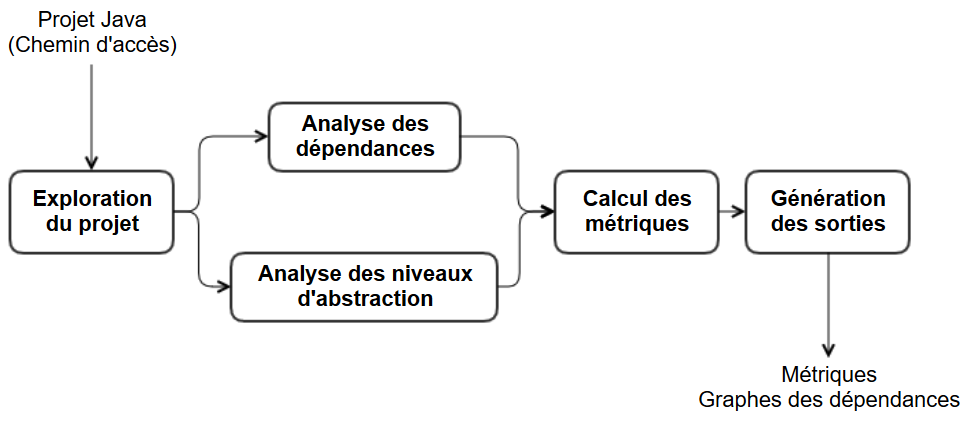
\includegraphics[width=\textwidth]{img/SimplifiedPipeline.png}    \caption{Pipeline de traitement de JMetrics}
    \label{fig:simplepipe}
\end{figure}

    \paragraph{}Afin que l'application atteigne son objectif d'obtention de métriques, il est nécessaire de passer par plusieurs étapes afin d'obtenir les informations nécessaires à leur calcul. On peut représenter ces différentes actions sous la forme d'un pipeline de traitement. En effet :

\begin{itemize}
	\item Chaque étape nécessite le résultat de la précédente afin de pouvoir être menée à bien.
	\item Aucun retour en arrière n'a lieu : une fois une action effectuée, il n'est plus nécessaire d'y revenir plus loin dans l'exécution.
\end{itemize}

    \paragraph{}La figure \ref{fig:simplepipe} illustre le pipeline dans les grandes lignes (il s'agit d'une version plus détaillée de la figure \ref{fig:intro} présente dans l'introduction). L'application est architecturée de manière à ce que chaque package ait la responsabilité de l'exécution d'une étape, chacune ne nécessitant qu'une interaction très limitée avec les autres. Ce pipeline se décompose en quatre phases principales :

    \begin{itemize}
        \bigbreak 
        \item[] \textbf{Exploration du projet (Package \texttt{project})} Dans un premier temps, l'application a besoin de construire une représentation exploitable du projet à analyser. Pour ce faire, celle-ci visite récursivement les répertoires et fichiers composant ce projet et crée un structure arborescente le représentant. La structure ainsi obtenue est ensuite nettoyée afin d'écarter les dossiers vides ou n'ayant que peut d'intérêt (par exemple un dossier n'en contenant qu'un autre).

        \bigbreak 
        \item[] \textbf{Analyse statique des classes (Package \texttt{analysis})} A partir des données précédemment générées, le programme parcourt toutes les classes référencées dans le projet et effectue une analyse de leur code (source ou bien compilé, en fonction du type d'analyse) afin d'en extraire les données nécessaires au calcul des métriques. Cette étape peut se scinder en deux sous-parties indépendantes et ayant la possibilité d'être effectuées en parallèle :
    	\begin{itemize}
    		\item \textit{Analyse du niveau d'abstraction} Il s'agit d'effectuer un comptage des méthodes composant la classe et d'en tirer deux valeurs : le \emph{nombre total de méthodes} et le \emph{nombre de méthodes abstraites} de la classe.
    		\item \textit{Analyse des dépendances} Cette seconde partie est la plus délicate des deux : il s'agit d'extraire les dépendances de la classe vis-à-vis des autres classes du projet. Cette analyse génère une \emph{liste de ces dépendances}.
    	\end{itemize}
	    A partir du résultat de l'analyse des dépendances, l'application génère un graphe pour représenter celles-ci.
	
	    \bigbreak 
	    \item[] \textbf{Calcul des valeurs des métriques (Package \texttt{metrics})} En utilisant les données renvoyées par l'étape d'analyse, l'application calcule différentes métriques (pour le moment : les métriques de Martin, mais avec possibilité d'extension) pour chaque classe, puis les classes sont regroupées en packages et les valeurs des métriques pour chacun d'eux sont calculées à partir des résultats précédents. Bien que ce ne soit pas le cas pour le moment, une approche similaire pourrait être envisagée pour d'autres niveaux de granularité.
	
	    \bigbreak 
	    \item[] \textbf{Présentation des résultats (Package \texttt{presentation})} Pour finir, les valeurs calculées précédemment doivent être présentées à l'utilisateur. Dans ce but, l'application génère plusieurs fichiers contenant les informations nécessaires (ex: graphe de dépendances au format DOT, tableau de métriques au format CSV, ...).
	
	\end{itemize}

    \paragraph{}Afin de faciliter la visualisation des données générées par l'application, plusieurs scripts \textit{Python} accompagnent l'application. Ils ne sont cependant que des aides, ne font pas partie du cœur de celle-ci et ne sont donc pas considérés comme une étape à part entière du pipeline. En outre, un cinquième package (\texttt{graph}) fait partie du projet mais n'a vocation qu'à fournir une structure de graphe partagées entre les autres packages. Il ne constitue donc pas une étape de traitement non plus.

\subsection{Organisation des composants}
\TODO{INSERT UML ON EACH PACKAGE}

\subsubsection{Package analysis}

    \paragraph{} Le package \textit{analysis} contient les composants chargés d'effectuer l'analyse statique du code des classes. Cette analyse est menée à bien par des parseurs. Il en existe deux catégories, chacune définie par une interface :
    \begin{itemize}
    	\item[\textbf{AbstractnessParser}, parseur d'abstraction.] Définit l'interface que doivent implémenter tous les parseurs ayant vocation à extraire les informations sur le niveau d'abstraction d'une classe (nombre de méthodes et nombre de méthodes abstraites).
    	\item[\textbf{CouplingParser}, parseur de dépendances.] Définit l'interface que doivent implémenter tous les parseurs qui récupèrent les dépendances d'une classe envers les autres.
    \end{itemize}
    Le parseur d'abstraction retourne un object de la classe \textbf{AbstractnessData}. Cette classe ne possède que deux attributs (numberOfMethods et numberOfAbstractMethods) et les \textit{getters} permettant d'y accéder. Le but de cette classe est uniquement d'encapsuler ces éléments.
    Le parseur de dépendances, quant à lui, retourne une liste d'objet de la classe \textbf{Dependency}. Cette classe a également pour but d'encapsuler les informations relatives à une dépendance (source, destination et type). Il s'agit d'une représentation intermédiaire avant la construction du graphe de dépendances.
    Dans son état actuel, l'application contient deux implémentations de chacune de ces interfaces : une permettant l'analyse sur du code source via \emph{l'API Eclipse JDT}\footnote{\url{https://help.eclipse.org/neon/index.jsp?topic=\%2Forg.eclipse.jdt.doc.isv\%2Freference\%2Fapi\%2Foverview-summary.html}} et l'autre servant à l'analyse du code compilé via l'API d'introspection de Java. Chaque implémentation est constituée de 3 classes :
    \begin{itemize}
    	\item Une implémentation d'AbstractnessParser. Il s'agit de \textbf{IntrospectionAbstractnessParser} pour l'introspection et \textbf{JDTAbstractnessParser} pour l'implémentation JDT.
    	\item Une implémentation de CouplingParser. Il s'agit de \textbf{IntrospectionCouplingParser} pour l'introspection et \textbf{JDTCouplingParser} pour l'implémentation JDT.
    	\item Une classe abstraite pour factoriser le code partagé. Il s'agit de \textbf{IntrospectionParser} pour l'introspection et \textbf{JDTParser} pour l'implémentation JDT.
	\end{itemize}
	L'implémentation utilisant le JDT a une particularité supplémentaire. En effet, l'API JDT faisant usage du pattern \emph{Visitor} pour parcourir le code source, les deux parseurs implémentent ce pattern. Il existe donc une méthode \emph{visit} pour chaque partie du code source permettant de récupérer les informations recherchées.
	
	\paragraph{} Afin de faciliter l'instanciation des parseurs par le code client, un interface \textbf{ParserFactory} est définie et implémentée pour fournir une \emph{factory} pour chacune des deux familles de parseurs (introspection et JDT) : \textbf{IntrospectionParserFactory} et \textbf{JDTParserFactory}. Pour le code client, il est nécessaire de passer par une factory car les constructeurs des parseurs ne sont disponibles que dans leur propre package.
	
	\paragraph{} Enfin, ce package définit également une énumération des types de dépendances (\textbf{DependencyType}) qui sont les suivants : \emph{Inheritance}, \emph{Aggregation} et \emph{UseLink}.
    
\subsubsection{Package graph}
    \TODO{TMP}
    \paragraph{}Le package \emph{graph} a pour objectif de mettre à disposition de l’application un graphe structurant un ensemble de dépendances et offrant différents algorithmes permettant d’effectuer des calculs sur ce graphe. Ce package est composé d’une classe principale \textbf{DirectedGraph} qui définit un graphe orienté comme structure de données.
    Le service (stateless) \textbf{GraphConstructor} est quand à lui charger de construire un graphe à partir d’un ensemble de Granule et d’un ensemble de dépendances entre ces granules. Elle assure également à partir  la représentation au format \emph{.dot} d'un graphe orienté.
    
    \TODO{En attente de validation} 
    La classe \emph{DirectedGraphEdge} définit la structure de donnée utilisée pour stocker les informations concernant les sommets (représenté par la classe \emph{DependencyEdge}) du graphe des dependances.

\subsubsection{Package metrics}
    \TODO{Quand on aura revu la structuration du package afin de s'assurer de sa flexibilité}


\subsubsection{Package presentation}
    \paragraph{}Le package \emph{presentation} fournit les classes nécessaires nous permettant de générer différents fichiers constituant des rapports d'analyse. Il existe deux types de représentation que nous avons mis en place, ces représentations sont définies par deux interfaces :
    \begin{itemize}
        \item \textbf{GraphPresentationBuilder} : Définit l'interface pour la construction de la représentation du graphe des dépendances sous la forme d'une chaîne de caractère qui représente le contenu du fichier \emph{.dot}
        \item \textbf{CSVRepresentable} : Définit l'interface qui va présenter dans un fichier \emph{.csv} le résultat des calculs des métriques pour chaque Granule. C'est dans cette classe Granule que l'on va implémenter les deux méthodes associées à cette interface. La première méthode va nous permettre de mettre en place la première ligne du fichier correspondant à la légende (nom du granule ainsi que les différentes métriques) puis dans la seconde méthode, elle va renseigner pour chaque granule le résultat du calculs des métriques. 
    \end{itemize}
    
     \TODO{Point 1 : A approfondir}
    
    La classe \textbf{CSVBuilder} va permettre la construction d'une chaîne de caractère au format CSV.
    L'implémentation de l'interface \textbf{GraphPresentationBuilder} sera réalisée par la classe \textbf{GraphDotBuilder} qui aura pour but de construire la représentation du graphe des dépendances dans le format \emph{.dot}
    
   La génération de ces deux formats de fichiers sont réalisées par l'intermédiaire de la classe \textbf{FileGenerator} 
   L'instanciation de cette classe est faite dans le \textbf{Main} où l'on génère les fichiers CSV et DOT pour chaque échelle de granularité.

    
\subsubsection{Package project}
	\paragraph{}Le package \emph{project} fournit les classes nécessaire à l'exploration d'un répertoire donnée et à la création d'une représentation de projet Java.

	\paragraph{}Le package est composé des trois éléments suivants :
	\begin{itemize}
		\item Une instance du pattern Composite permet de représenter l’arborescence des composants du projet. Une classe mère \texttt{ProjectComponent} maintient une référence en tant qu’attribut vers un objet \texttt{File}. Les packages sont représentés par la classe Composite \texttt{PackageDirectory} exposant un ensemble de \texttt{ProjectComponent}. Les classes sont représentées par la classe Feuille \texttt{ClassFile} exposant un \emph{stream}.
		\item La \texttt{ProjectStructure} est une classe Singleton qui conserve en mémoire la structure du projet qui s’apprête à être analysé et qui fournit des méthodes permettant l’accès aux différents composants du projets (classes et packages). Elle représente un repository.
		\item Enfin, le \texttt{FileSystemExplorer} est un service qui a pour objectif de construire la représentation du projet au travers de l'exploration du système de fichier et d’affecter la racine de celle-ci dans la classe Singleton. 
	\end{itemize}
	\TODO{Dernier point itemize : Parler de la structure FileSystemExplorer (Source / Bytecode).}
    La structure du projet est construite, lue et parcourue au travers d’algorithmes récursifs.
    
    



\subsection{Choix d'implémentation}

    \subsubsection{Comparaison des méthodes d'analyse}
    \label{methodsComparison}
    \paragraph{} Il existe deux méthodes pour analyser un programme Java : l'analyse de bytecode et l'analyse de code source. Le but de cette section est de dresser une comparaison entre celles-ci.
    
    \paragraph{Informations récupérables} Tout d'abord, le code source contient des informations perdues à la compilation et qui ne peuvent donc pas être retrouvées dans le bytecode. En effet, toutes les informations liées aux types génériques sont effacées car elles ne sont utilisées que dans le but d'effectuer des vérifications à la compilation, empêchant par là la détection de certaines dépendances.
    
    Par exemple, si on dispose du programme suivant :
    
    \begin{minipage}{(\textwidth/2) - 0.6cm}
        \begin{lstlisting}
public class A {

}
        \end{lstlisting}
    \end{minipage}
    \hspace{0.5cm}
    \begin{minipage}{(\textwidth/2) - 0.6cm}
        \begin{lstlisting}
public class B {
    private List<A> aList;
}
        \end{lstlisting}
    \end{minipage}
    
    On remarque que B possède une liste de A (il s'agit donc d'une dépendance d'association, B ayant une agrégation de A). Lorsque l'analyse passera sur l'attribut \texttt{aList}, on s'attend à ce que son type soit \texttt{List<A>} afin de pouvoir extraire la dépendance vers A. Si on effectue l'analyse sur le code source, on obtient effectivement ce résultat. Si cependant on analyse le bytecode du même programme, le type de \texttt{aList} sera uniquement \texttt{List}, l'information de généricité du type \texttt{List} étant effacée à la compilation. En utilisant la méthode analysant le bytecode, aucune dépendance de B vers A ne sera donc détectée sur ce programme. L'analyse de code source n'a pas cette limitation car les informations de types génériques y sont écrites.
    
    Certaines autres indications sont également absentes du bytecode : la déclaration de nom de package (bien que récupérable depuis le nom complet de la classe), les déclarations \textit{import}, ... . Ceci n'est pas gênant car l'application n'exploite pas ces informations.
    
    \paragraph{Outils et facilité de mise en place} Il existe plusieurs outils/bibliothèques permettant d'exploiter l'une des deux méthodes :
        \begin{itemize}
            \item[\textbf{Bytecode}] Les principales bibliothèques sont les suivantes :
            \begin{itemize}
                \item[\textit{API java.reflect}\footnotemark]\footnotetext{\url{https://docs.oracle.com/javase/8/docs/api/java/lang/reflect/package-summary.html}} L'introspection est la manière la plus rapide d'extraire des données depuis un code compilé car il s'agit d'une API directement intégrée au JDK. Le chargement des classes est facile et le parcours des attributs et méthodes également. Il est cependant plus difficile de charger une classe et l'analyser via cet API si cette même classe est déjà chargée dans la JVM et que les versions diffèrent (par exemple, si on analyse l'API Java 5 en lançant le locigiel sur un JVM Java 8 : beaucoup de classes déjà chargée en mémoire portent le même nom mais comportent énormément de différences). Ceci est dû au fait que pour récupérer des informations sur un classe via l'introspection, il est nécessaire de la charger dans la JVM comme s'il s'agissait d'une classe faisant partie de notre logiciel. En outre, cette API ne permet pas l'accès au corps des méthodes, empêchant par là même l'extraction de la grande majorité des dépendances de liens d'usage.
                \item[\textit{ASM}\footnotemark] \footnotetext{\url{https://asm.ow2.io/}}La bibliothèque permettant l'analyse (et même la modification) de bytecode la plus populaire est ASM. Cette dernière, contrairement à l'introspection, ne nécessite pas de charger les classes dans le JVM et permet l'accès aux instructions situées dans le corps des méthodes. Il s'agit cependant d'une bibliothèque externe et son utilisation nécessite d'implémenter certaines de ses interfaces (en suivant notamment le pattern Visitor) afin d'accéder au code, ce qui rend son adoption un peu moins rapide que celle de l'introspection. Cependant, elle permet d'extraire toutes les informations contenues dans le bytecode, permettant ainsi de récupérer la plupart des dépendances.
            \end{itemize}
            \item[\textbf{Code source}] Les principales bibliothèques sont les suivantes :
            \begin{itemize}
            	\item[\textit{Eclipse JDT}] La bibliothèque JDT, faisant partie du projet Eclipse, est l'API de parsing de code Java la plus populaire. A partir de code source Java, JDT construit un arbre de syntaxe abstrait (AST) qui peut ensuite être parcouru (en suivant le pattern Visitor) afin d'effectuer certaines actions sur les nœuds correspondant à des instructions qui nous intéressent. Cette bibliothèque existe depuis longtemps, est très activement maintenue par bon nombre de développeurs et possède un support complet des spécifications de toutes les versions du langage Java (de 1 à 11). Elle présente cependant deux points faibles : sa difficulté à mettre en place et sa relative lenteur. En effet, afin d'utiliser des fonctionnalités avancées de JDT, il faut faire appel à plusieurs autres API du projet Eclipse. De plus, de par sa grande complexité en terme de fonctionnalités offertes, JDT prend du temps et de la mémoire pour parser un grand nombre de fichiers source et à construire leur AST quand on veut résoudre tous les liens existant entre les symboles (par exemple entre l'instanciation d'une classe et sa déclaration).
            	\item[\textit{JavaParser}\footnotemark] \footnotetext{\url{https://javaparser.org/}} JavaParser est une autre API de parsing de code source Java, la deuxième plus populaire après JDT. Elle est également activement maintenue, supporte toutes les versions de Java de 1 à 11 et a un fonctionnement similaire à JDT : elle construit un AST à partir du code source Java et permet le parcours de celui-ci via une implémentation du pattern Visitor. La construction des AST est plus rapide qu'avec JDT, mais JavaParser semble ne pas pouvoir résoudre tous les liens dans le code. Son utilisation est cependant plus aisée car il n'est pas nécessaire de faire appel à d'autres API pour accéder aux fonctionnalités plus avancées.
            \end{itemize}
        \end{itemize}
        
        \TODO{Reformuler paragraph suivant (titre et contenu). Propal : Remarques annexes}
        \paragraph{Avantages et inconvénients divers} Il existe quelques différences supplémentaires dont le poids au sein du comparatif est moindre par rapport à celles citées au cours des paragraphes précédents :
        \begin{itemize}
        	\item[\textbf{Complexité en temps}] Quel que soit l'outil utilisé, il est plus rapide d'effectuer une analyse de bytecode qu'une analyse de code source. Cela est dû au fait que beaucoup de liens sont résolus à la compilation et ne nécessitent pas d'être recalculés (par exemple, lors de l'instanciation d'une classe, on connaît directement son nom complet) là où les parseurs de code source doivent les construire.
        	\item[\textbf{Disponibilité des fichiers}] Bien que cela survienne très rarement, il est possible que l'utilisateur veuille analyser l'architecture d'une application dont il ne possède que les fichiers de code compilé. Dans ce cas, l'analyse de code source ne peut se faire (où alors il faut décompiler le code, procédé assez délicat) et il faut impérativement utiliser l'analyse de code compilé. Dans le cas contraire (le plus courant), on ne possède que le code source. On peut alors obtenir le bytecode aisément en compilant le programme. Il est donc possible d'utiliser autant l'analyse de code source que l'analyse de bytecode.
        \end{itemize}
        \TODO{Add : Transformation structurelle du code}
        
    \subsection{Évolution du projet}
        \paragraph{}Compte rendu des rendez vous :
        \begin{center}
            \url{https://www.overleaf.com/6275561163kpwqmsbgmdzw}
        \end{center}
        
    
    
% Évolution du projet, Détails...
    

\newpage
\section{Tests}
    \paragraph{}Nous avons — tout au long de notre projet — développé une série de tests permettant de contrôler le bon fonctionnement de notre implémentation. Les outils et méthodes que nous avons utilisés ayant évolué au cours de la période de développement, ces tests nous ont permis d'identifier les problèmes de régression. Enfin, au travers de la mise en œuvre des tests directement liés à notre domaine d’étude (analyse et métrique), nous avons pu appréhender les spécificités et ainsi améliorer le cœur de notre programme.
    
    \paragraph{}Les composants de notre application ayant été soumis à une série de tests sont les suivants : 
    \begin{itemize}
    	\item Le parcours du FileSystemExplorer et la création de ProjectStructure.
    	\item Le classe Metrics et les différents calculs attachés.
    	\item Le graphe, ses primitives ainsi que les services qui y sont associés.
    	\item L’analyse de code.
    \end{itemize}

\subsection{Infrastucture de test}

    \paragraph{}Pour la mise en oeuvre de ces tests, nous avons utilisé le framework \textbf{JUnit 5}.
    
    \paragraph{Vérité terrain}Le package \texttt{analysis} ne pouvant pas être testé de manière triviale, nous avons mise en oeuvre une \textbf{vérité terrain annotée} qui nous a permis de vérifier la bonne concordance des données de dépendances et des données d’abstraction extraites par notre application avec les données réellement présentes dans un projet Java.
    
    Cette vérité terrain est constituée d’un ensemble de projet Java présentant des cas divers de dépendances et d'abstraction. Nous avons mis en place un système d’annotation Java permettant de simplifier la saisie et la création d'éléments de cette vérité terrain.
    
    \TODO{Integrate example code annotation}
    \TODO{TMP: Actuellement en complétion}
    
    \paragraph{}Une classe \texttt{GroundTruthManager} a pour but de charger en mémoire les différents projets composants la vérité terrain et offre des méthodes d'accès à ces différentes données. Le code des tests de nos parsers est ainsi simplifier : le parcours de la vérité terrain vérifie la conformité des données d'annotation au données extraites par nos parsers.

\subsection{Tests unitaires}

\subsection{Tests d'intégration}

\subsection{Tests de performance}

    \paragraph{}Nous avons effectué des tests de performance. Ces derniers ont consisté en l’exécution de l’application sur des projets Java plus ou moins largse (dont notamment l'API Java lui-même). Ces tests nous ont permis d’obtenir un tableau représentatif des performances de notre application.

    \paragraph{}Les tests de performance ont été effectués sur la configuration suivante :
    \begin{itemize}
        \item Ordinateur portable Asus Zenbook Pro 15
        \item \textbf{Java} : Oracle JRE 1.8 revision 201 (Win x64)
        \item \textbf{Système d'exploitation} : Windows 10 v. 1809
        \item \textbf{Processeur} : i7 8750H 4.1Ghz
        \item \textbf{RAM} : 16Go DDR4
    \end{itemize}
    
    \paragraph{}Nous obtenons les données suivantes : 
    \begin{center}
        \begin{tabular}{|c|c|c|c|}\hline
            Projet & Nombre de classes & Nombre de packages & Temps d'exécution \\ \hline
            Oracle JDK 1.8 & 7651 & 486 & 12 min 42 s \\ \hline
            JUnit 5 & 435 & 58 & 0 min 19 sec \\ \hline
            JMetrics & 41 & 6 & 0 min 2 sec \\ \hline
        \end{tabular}
    \end{center}

    \TODO{Les tests mis en échec (Ce qui ne passe pas)}


\subsection{Tests de fonctionnement}
    \TODO{Comparaison avec résultat présents dans l'article des suédois et les résultats d'analyse JDepend}

\newpage
\section{Résultats \& Interprétations}

    \paragraph{Données extraites}A l'exécution de notre application, plusieurs fichiers sont générés (au format CSV et DOT) permettant d'extraire les données de l'analyse. Ces données sont les mesures de dépendances sous formes de graphe (représentation graphique ou matricielle) ou de liste ; et les données de métriques :
    \begin{itemize}
        \item \textbf{Graphe des dépendances} : En récupérant les dépendances associées à chaque granule, il nous a été possible de générer un fichier au format \emph{.dot} nous affichant un graphe de dépendance. 
        \item \textbf{Valeurs des métriques} : Le résultat du calcul des métriques a été écrit dans un fichier au format \emph{.csv} où sont référencés pour chaque granule, son nom, ses valeurs de Ca, Ce, I, A et Dn.
    \end{itemize}
    \paragraph{}Ces données sont classés par niveau de granularité (\emph{class scale} et \emph{package scale}).

    \subsection{Présentation}

    \paragraph{Représentation proposés}Afin d'offrir à l'utilisateur des outils d'interprétation des données bruts extraites par notre analyse, nous avons mise en place une série de scripts Python basé sur la lecture des fichiers csv extraits. Nous étudierons ici le programme \textcolor{red}{X} à la granularité des packages. Les différentes représentations proposées sont les suivantes :
    \TODO{INSERT PLOT ON EACH REPRESENTATION}

        \begin{itemize}
        \item \textbf{Histogramme (Stabilité)}
        \item \textbf{Histogramme (Dépendances)} : Cette représentation nous permet d'étudier le poids des types de dépendances dans la valeur de couplage et donc de stabilité des différents granules. L'histogramme ne permet pas de représenter les données de couplage afférent et efférent (1 seul axe étant disponible pour l'affichage de valeur). C'est pour cette raison que nous étudions les données de couplages général depuis une autre représentation décrite ci-dessous.

        \item \textbf{Représentation 2D (Instabilité et Abstraction)} : Nous avons mis en place une représentation mettant en relation la donnée d'instabilité et d'abstraction sur un axe orthogonal. Cette représentation permet d'afficher les différents granules en fonction de leur stabilité et de leurs niveau d'abstraction. 
        A l'image de ce que décrit Martin dans son article nous positionnons sur le plan les zones de souffrance et d'inutilité ainsi que la séquence principale. 
        
        En survolant un point du plan, il est possible d'obtenir les coordonnées du plan (données d'abstraction et de stabilité), la distance du point à la séquence principale et la liste des granules présents sur la position.
        
        Cette représentation graphique, bien que soumise a certaine critique est très représentative de la métrique énoncé par Martin. Elle permet de visualiser directement les données d'abstraction, de stabilité et de distance.

        \item \textbf{Représentation 2D (Couplage afférent et efférent)}Nous avons mis en place une représentation mettant en relation les données de couplage afférent et efférent sur un axe orthogonal. Cette représentation nous permet d'étudier la stabilité en séparant la propriété de responsabilité et d'indépendance. De plus, elle nous permet d'étudier les extréma des valeurs de couplage. Nous faisons ici abstraction de la donnée type de dépendances pour nous concentrer sur la donnée de couplage uniquement.
    \end{itemize}
    
    
    \TODO{Parler de la visualisation de Martin sur l'évolution de D selon les releases : cf. p.267 Martin's Book}

    

    \subsection{Expérimentation : Analyze GoF's Design Pattern}
    \TODO{Nous avons --- conjointement à l'unité d'enseignement PDP --- une unité d'enseignement Architecture logicielle dans laquelle nous découvrons les Design Pattern exposé par Gamma, x, x, x[refBib]. Nous avons souhaiter créer une passerelle entre ces 2 UEs en produisant l'analyse des différents design pattern par notre programme. La motivation ayant mené à l'élaboration des design patterns étant une "architecture propre/low-coupling/etc." (terme tmp), nous avons jugé cette analyse pertinente.}
    
    \TODO{Interprétations de résultats}




\newpage
\section{Conclusion et perspective}
    \subsection{Bilan, ce qui a été fait}
    \subsection{Perspective, ce qu'on pourrait faire}



% ----------> BIBLIOGRAPHY
\pagebreak
\bibliographystyle{unsrt}
\bibliography{references}


\newpage
\begin{appendices}


\section{Exemple de projet annoté}
\TODO{Corriger exemple}
    \paragraph{}Dans le but de vérifier que l'application calcule les valeurs de métrique correctement, il est nécessaire d'écrire de petits logiciels simples présentant des configurations de dépendances différentes. Nous donnons ici un exemple élémentaire de projet annoté.
    
\begin{minipage}{7.5cm}
\begin{lstlisting}[caption=Classe Vehicle]
public abstract class Vehicle {
    private int nbWheel;
    private ArrayList<Wheel> wheels;
    public abstract void move();
    public void setNbWheel(int i) { }
    public void addWheel(Wheel w) { }
}
\end{lstlisting}
\end{minipage}
\hspace{0.5cm}
\begin{minipage}{6cm}
\begin{lstlisting}[caption=Enumeration Material]
public enum Material {
    Plastic,
    Metal,
    Carbon
}
\end{lstlisting}
\end{minipage}
\vspace{0.5cm}
\begin{lstlisting}[caption=Classe Airplane]
public class Airplane extends Vehicle {
    @Override
    public void move() { /* ... */ }
}
\end{lstlisting}
\begin{lstlisting}[caption=Classe Car]
public class Car extends Vehicle {
    @Override
    public void move() { /* ... */ }
}
\end{lstlisting}
\begin{lstlisting}[caption=Classe Wheel]
public class Wheel {
    private Material material;
    public Material getMaterial() { return this.material; }
    public void setMaterial(Material m) { this.material = m; }
}
\end{lstlisting}



\begin{figure}[h!]
    \centering
    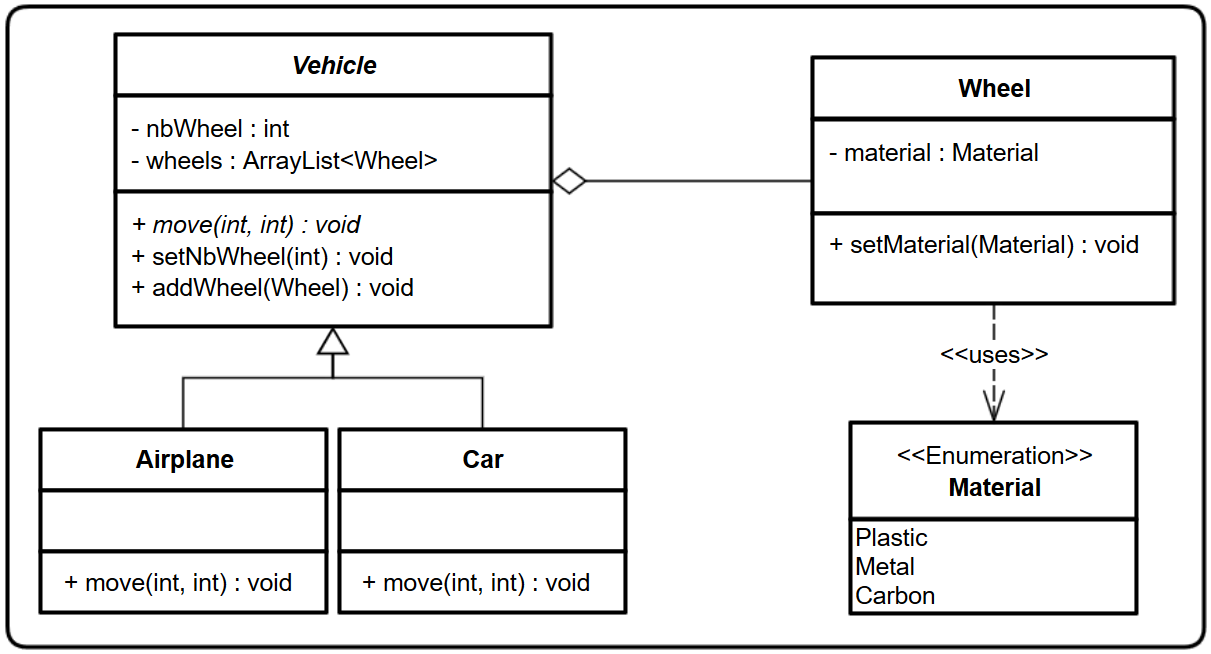
\includegraphics[scale=0.5]{img/uml_example.png}
    \caption{Diagramme de classe du projet exemple}
\end{figure}


\begin{table}[H]\caption{Tableau exposant les métriques}
    \centering
    \begin{tabular}{|c|c|c|c|c|c|}
        \hline
        \textbf{Catégorie} & \textbf{Ca} & \textbf{Ce} & \textbf{A} & \textbf{I} & \textbf{Dn} \\
        \hline
        \textbf{Vehicle} & 2 & 1 & 0.33 & 0.33 & 0.33 \\
        \hline
        \textbf{Material} & 1 & 0 & 0 & 0 & 1 \\
        \hline
        \textbf{Airplane} & 0 & 1 & 0 & 1 & 0  \\
        \hline
        \textbf{Car} & 0 & 1 & 0 & 1 & 0 \\
        \hline
        \textbf{Wheel} & 1 & 1 & 0 & 0.5 & 0.5 \\
        \hline
    \end{tabular}
\end{table}


\begin{figure}
    \centering
    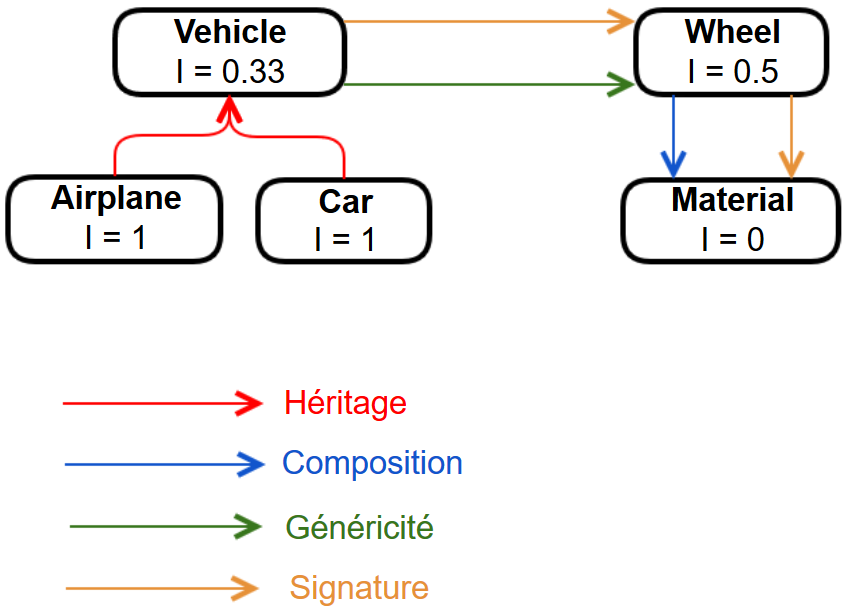
\includegraphics[scale=0.5]{img/gdd_example.png}
    \caption{Graphe des dépendances du projet exemple}
\end{figure}

\end{appendices}


\end{document}
